\documentclass[25pt, a0paper, landscape]{tikzposter}
\tikzposterlatexaffectionproofoff

% support for LuaTeX => striclty better
%
% most things stated for LuaTeX also apply for XeTeX, but XeTeX is not
% very useful now, since LuaTeX is widely available
\usepackage{ifluatex}
\ifluatex
% use the CI font of TUM
% download from mytum portal (search for TUM CI/CD stuff)
% the scaling is the default from TUM templates
\usepackage{fontspec}
%\setsansfont{TUM Neue Helvetica}[Scale=0.95]
%\setmainfont{TUM Neue Helvetica}[Scale=0.95] % use TUM font (not a nice one)
\setmainfont{Dosis}
\usepackage{polyglossia}
\setdefaultlanguage{english}
\else
% only needed for oldschool TeX Enginge
\usepackage[utf8]{inputenc}     % does not work with LuaTeX
\usepackage[english]{babel}     % does not work well with LuaTeX
\fi

\usepackage[final]{microtype}   % improve typography, e.g. kerning

\usepackage{subcaption}
\AtBeginEnvironment{tikzfigure}{\captionsetup{type=figure}}


\usepackage{authblk}
\makeatletter
\renewcommand\maketitle{\AB@maketitle} % revert \maketitle to its old definition
\renewcommand\AB@affilsepx{\quad\protect\Affilfont} % put affiliations into one line
\makeatother
\renewcommand\Affilfont{\Large} % set font for affiliations

\usepackage{amsmath, amsfonts, amssymb}
\usepackage{tikz}
\usepackage{pgfplots}

% align columns of tikzposter; needs two compilations
\usepackage[colalign]{column_aligned}

% tikzposter meta settings
% \usetheme{Default}
% \usetitlestyle{Default}
% \useblockstyle{Default}
\usetheme{Simple}

\definetitlestyle{Team9Title}{
    width=600mm, roundedcorners=30, linewidth=0.4cm, innersep=1cm,
    titletotopverticalspace=15mm, titletoblockverticalspace=20mm,
    titlegraphictotitledistance=10pt, titletextscale=1
}{
    \begin{scope}[line width=\titlelinewidth, rounded corners=\titleroundedcorners]
        \draw[draw=none, fill=titlebgcolor]%
        (\titleposleft,\titleposbottom) rectangle (\titleposright,\titlepostop);
    \end{scope}
}

\usetitlestyle{Team9Title}


\defineblockstyle{Team9Blocks}{
    titlewidthscale=1, bodywidthscale=1, titleleft,
    titleoffsetx=0pt, titleoffsety=0pt, bodyoffsetx=0pt, bodyoffsety=0pt,
    bodyverticalshift=0pt, roundedcorners=0, linewidth=0.2cm,
    titleinnersep=1cm, bodyinnersep=1cm
}{
    \begin{scope}[line width=\blocklinewidth, rounded corners=\blockroundedcorners]
      % \draw[draw=framecolor]%, fill=blockbodybgcolor]
      % (blockbody.south west) rectangle (blocktitle.north east);      
      \draw[draw=framecolor]
        (blockbody.south west) rectangle (blockbody.north east);
      \ifBlockHasTitle %
           \draw[color=blocktitlebgcolor]
               (blocktitle.south west) -- (blocktitle.south east);%
       \else
        \fi
    \end{scope}
}

\useblockstyle{Team9Blocks}

% color handling
\definecolor{TumBlue}{cmyk}{1,0.43,0,0}
\colorlet{blocktitlebgcolor}{TumBlue!50}
\colorlet{blocktitlefgcolor}{TumBlue}
\colorlet{blockbodybgcolor}{TumBlue!50}
\colorlet{framecolor}{TumBlue!50}
\colorlet{backgroundcolor}{white}

\colorlet{titlebgcolor}{TumBlue}
%\colorlet{titlebgcolor}{}


%%%%%%%%%%% redefine title matter to include one logo on each side of the title; adjust with \LogoSep
\makeatletter
\newcommand\insertlogoi[2][]{\def\@insertlogoi{\includegraphics[#1]{#2}}}
\newcommand\insertlogoii[2][]{\def\@insertlogoii{\includegraphics[#1]{#2}}}
\newlength\LogoSep
\setlength\LogoSep{-70pt}

\renewcommand\maketitle[1][]{  % #1 keys
    \normalsize
    \setkeys{title}{#1}
    % Title dummy to get title height
    \node[inner sep=\TP@titleinnersep, line width=\TP@titlelinewidth, anchor=north, minimum width=\TP@visibletextwidth-2\TP@titleinnersep]
    (TP@title) at ($(0, 0.5\textheight-\TP@titletotopverticalspace)$) {\parbox{\TP@titlewidth-2\TP@titleinnersep}{\TP@maketitle}};
    \draw let \p1 = ($(TP@title.north)-(TP@title.south)$) in node {
        \setlength{\TP@titleheight}{\y1}
        \setlength{\titleheight}{\y1}
        \global\TP@titleheight=\TP@titleheight
        \global\titleheight=\titleheight
    };

    % Compute title position
    \setlength{\titleposleft}{-0.5\titlewidth}
    \setlength{\titleposright}{\titleposleft+\titlewidth}
    \setlength{\titlepostop}{0.5\textheight-\TP@titletotopverticalspace}
    \setlength{\titleposbottom}{\titlepostop-\titleheight}

    % Title style (background)
    \TP@titlestyle

    % Title node
    \node[inner sep=\TP@titleinnersep, line width=\TP@titlelinewidth, anchor=north, minimum width=\TP@visibletextwidth-2\TP@titleinnersep]
    at (0,0.5\textheight-\TP@titletotopverticalspace)
    (title)
    {\parbox{\TP@titlewidth-2\TP@titleinnersep}{\TP@maketitle}};

    \node[inner sep=0pt,anchor=west] 
    at ([xshift=-\LogoSep]title.west)
    {\@insertlogoi};

    \node[inner sep=0pt,anchor=east] 
    at ([xshift=\LogoSep]title.east)
    {\@insertlogoii};

    % Settings for blocks
    \normalsize
    \setlength{\TP@blocktop}{\titleposbottom-\TP@titletoblockverticalspace}
}
\makeatother
%%%%%%%%%%%%%%%%%%%%%%%%%%%%%%%%%%%%%


\usepackage{url}

% graphics
\graphicspath{{../logs/results/},{results/}}

\let\thempfootnote\thefootnote%http://tex.stackexchange.com/questions/956/footnotemark-and-footnotetext-in-minipage#959
\newcommand\printfootnote[1]{% to get different numbers for different footnotes
  \addtocounter{footnote}{1}%
  \footnotetext{#1}}

% title matter
\title{Image Super--Resolution with GANs}

\author[1]{Nathanael Bosch}
\author[1]{Thomas Grassinger}
\author[1]{Jonas Kipfstuhl}
\author[1]{Pierre Springer}

% remove the ugly 'and' before last author, as a benefit Pierre is in line again
\renewcommand{\Authands}{, }

% define a length for the heigt of the images
\newlength{\imageheight}
\setlength{\imageheight}{16cm}

\affil[1]{Technical University of Munich}

\insertlogoi[width=15cm]{tum_logo}
\insertlogoii[width=15cm]{tum_logo}


% main document
\begin{document}

\maketitle

\begin{columns}
  
  % Introduction and explanation of GANs
  \column{0.4}

  \block{Introduction}{%
    We call super-resolution (SR) the task of estimating a
    high-resolution (HR) image from its low-resolution (LR)
    counterpart.\\
    Recent work with optmizition-based methods largely
    focuses on minimizing the mean squared reconstruction error. This
    results in high peak signal-to-noise ratios, but they often have
    problems with modelling high-frequency details. The results are
    often too smooth. In our work we tried to tackle this problem
    using generative adversarial networks (GANs).
  }
  
  \block{GANs}{%
GANs consist of two different networks, a Generator Network and a
Discriminator Network. The concept behind this is that the generative
network estimates a super-resolved image from its LR version with the
goal to become highly similar to real images that the discriminator
network fails to distiguish.

Therefore we optimize the discriminator network $D_{\Theta_D}$ in an
alternating manner along with the generative network $G_{\Theta_G}$ to
solve the adversarial min-max problem:
\begin{align*}
  \min_{\Theta_G} \max_{\Theta_G} \mathbb{E}_{I^{HR} \backsim p_{\text{train}}(I^{HR})}
  [\text{log} D_{\Theta_D}(I^{HR})]+\mathbb{E}_{I^{HR} \backsim p_G(I^{LR})}
[\text{log} (1-G_{\Theta_G}(I^{LR}))]
\end{align*}

\begin{tikzfigure}[h]
  \centering
  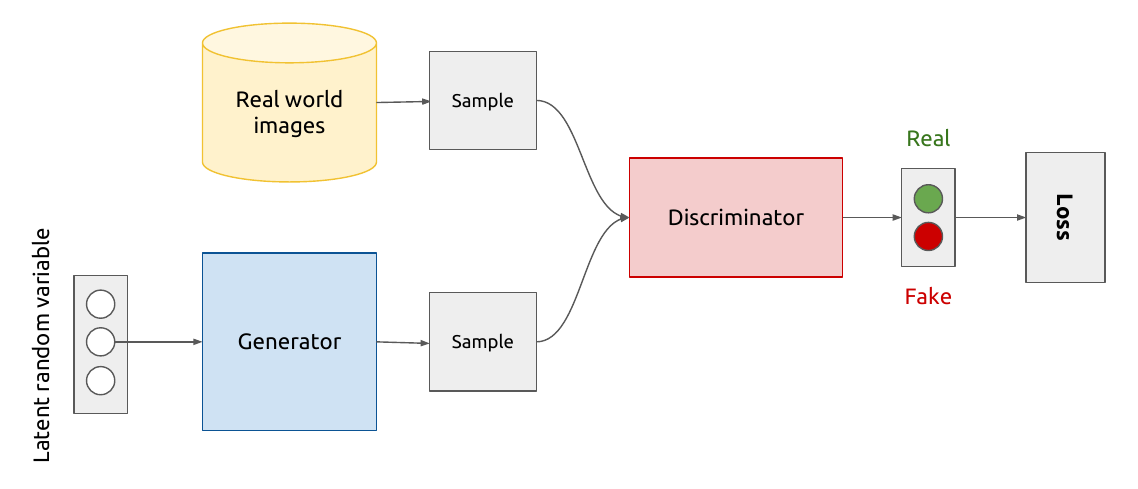
\includegraphics[width=\linewidth]{gan.png}
\end{tikzfigure}

  The perceputal loss $l^{SR}$ we defined as weighted sum of a content loss and an discriminative loss component:
  \begin{equation*}
    l^{SR}=\alpha l^{SR}_{MSE} + \beta l^{SR}_{VGG16_19/i.j} + \gamma l^{SR}_{D}
  \end{equation*}
  Where $l^{SR}_{MSE}$ is a mean squared error term, $l^{SR}_{VGG}$ is
  an euclidean distance of the VGG feature representation for the
  images, and $l^{SR}_{D}$ is the discriminative loss.
  
  % More precisely, the content loss components are defined as follows:\\
  % $l^{SR}_{MSE}= \frac{1}{r^2WH}\sum_{x=1}^{rW}\sum_{y=1}^{rH}(I^{HR}_{x,y}-G_{\theta_G}(I^{LR})_{x,y})^2$\\
  % $l^{SR}_{VGG1619/i.j}={\frac{1}{W_{i,j}H_{i,j}} \sum_{x=1}^{W_{i,j}}\sum_{y=1}^{H_{i,j}}(\Phi_{i,j}(I^{HR})_{x,y}-\Phi_{i,j}(G_{\Theta_G}(I^{LR}))_{x,y}}^2$\\
  % the discriminative loss as follows\\
  % $l^{SR}_{D}=\sum_{n=1}^N
  % -\text{log}D_{\Theta_D}(G_{\Theta_G}(I^{LR}))$

  
% \\ \\ min$_{\Theta_G}$ max$_{\Theta_G}$
% $\mathbb{E}_{I^{HR} \backsim p_{\text{train}}(I^{HR})} [\text{log}
% D_{\Theta_D}(I^{HR})]+\mathbb{E}_{I^{HR} \backsim p_G(I^{LR})}
% [\text{log} (1-G_{\Theta_G}(I^{LR}))]$\\ %schaut bisschen komisch aus
% mit der Formel über die 2 Seiten \\ %(den Satz mit der Formel würde
% ich auf dem Poster rauslassen, außerdem auf die Netzwerk Architektur
% der beiden Netze nicht näher eingehen (sind halt deep nets mit conv
% layern))

% The perceputal loss $l^{SR}$ we defined as weighted sum of a content
% loss and an discriminative loss component:\\ $l^{SR}=\alpha
% l^{SR}_{MSE} + \beta l^{SR}_{VGG16_19/i.j} + \gamma l^{SR}_{D}$\\ More
% precisely, the content loss components are defined as follows:\\
% $l^{SR}_{MSE}=
% \frac{1}{r^2WH}\sum_{x=1}^{rW}\sum_{y=1}^{rH}(I^{HR}_{x,y}-G_{\theta_G}(I^{LR})_{x,y})^2$\\
% $l^{SR}_{VGG1619/i.j}={\frac{1}{W_{i,j}H_{i,j}}
% \sum_{x=1}^{W_{i,j}}\sum_{y=1}^{H_{i,j}}(\Phi_{i,j}(I^{HR})_{x,y}-\Phi_{i,j}(G_{\Theta_G}(I^{LR}))_{x,y}}^2$\\
% the discriminative loss as follows\\ $l^{SR}_{D}=\sum_{n=1}^N
% -\text{log}D_{\Theta_D}(G_{\Theta_G}(I^{LR}))$\\
}

\block{Datasets}{
  \begin{description}
  \item[PASCAL VOC\footnotemark{}] over 10\,000 images for
    classification in 20 categories
  \item[NITRE\footnotemark{}] 800 high resolution images
  \end{description}

}


  % our results
  \column{0.6}

  % divide for plots and images
  \block{Results}{

    \begin{tikzfigure}
      \subcaptionbox{VGG1619 perceptual, adversarial, image loss}[0.18\linewidth]{%
        \includegraphics[width=0.33\linewidth, height=\imageheight, keepaspectratio]{vgg1619_p_a_i}
      }
      \subcaptionbox{VGG1619 perceptual, adversarial loss}[0.18\linewidth]{%
        \includegraphics[width=\linewidth, height=\imageheight, keepaspectratio]{vgg1619_p_a}
      }
      \subcaptionbox{VGG1619 perceptual, image loss}[0.18\linewidth]{%
        \includegraphics[width=\linewidth, height=\imageheight, keepaspectratio]{vgg1619_p_i}
      }
      \subcaptionbox{VGG1619 perceptual loss}[0.18\linewidth]{%
        \includegraphics[width=\linewidth, height=\imageheight, keepaspectratio]{vgg1619_p}
      }
      \subcaptionbox{VGG1619 adversarial, image loss}[0.18\linewidth]{%
        \includegraphics[width=\linewidth, height=\imageheight, keepaspectratio]{vgg1619_a_i}
      }
    \end{tikzfigure}

    \begin{tikzfigure}
      \subcaptionbox{VGG1619 adversarial loss}[0.18\linewidth]{%
        \includegraphics[width=\linewidth, height=\imageheight, keepaspectratio]{vgg1619_a}
      }
      \subcaptionbox{VGG1619 image loss}[0.18\linewidth]{%
        \includegraphics[width=\linewidth, height=\imageheight, keepaspectratio]{vgg1619_i}
      }
      \subcaptionbox{VGG19 perception, adversarial, image loss}[0.18\linewidth]{%
        \includegraphics[width=\linewidth, height=\imageheight, keepaspectratio]{vgg19_p_a_i}
      }
      \subcaptionbox{VGG16 perception, adversarial, image loss}[0.18\linewidth]{%
        \includegraphics[width=\linewidth, height=\imageheight, keepaspectratio]{vgg16_p_a_i}
        }
    \end{tikzfigure}
  }
  
  % \begin{subcolumns}
  %   \subcolumn{0.5}
  %   \block{Statistics2}{%
  %     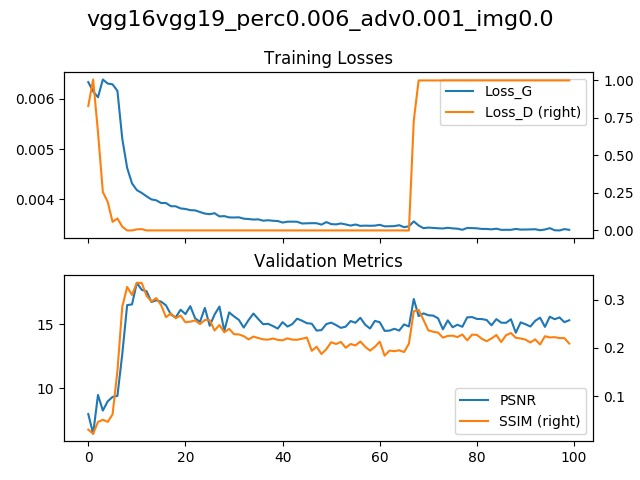
\includegraphics[width=\linewidth, height=\imageheight, keepaspectratio]{vgg16cgg19stats.jpeg}%
  %     % Some plots for clarifying the performance and distinguishing different Network models, e.\,g., VGG16, VGG19.
  %   }
    
  %   % images column
  %   \subcolumn{0.5}
  %   \block{Results2}{%
  %     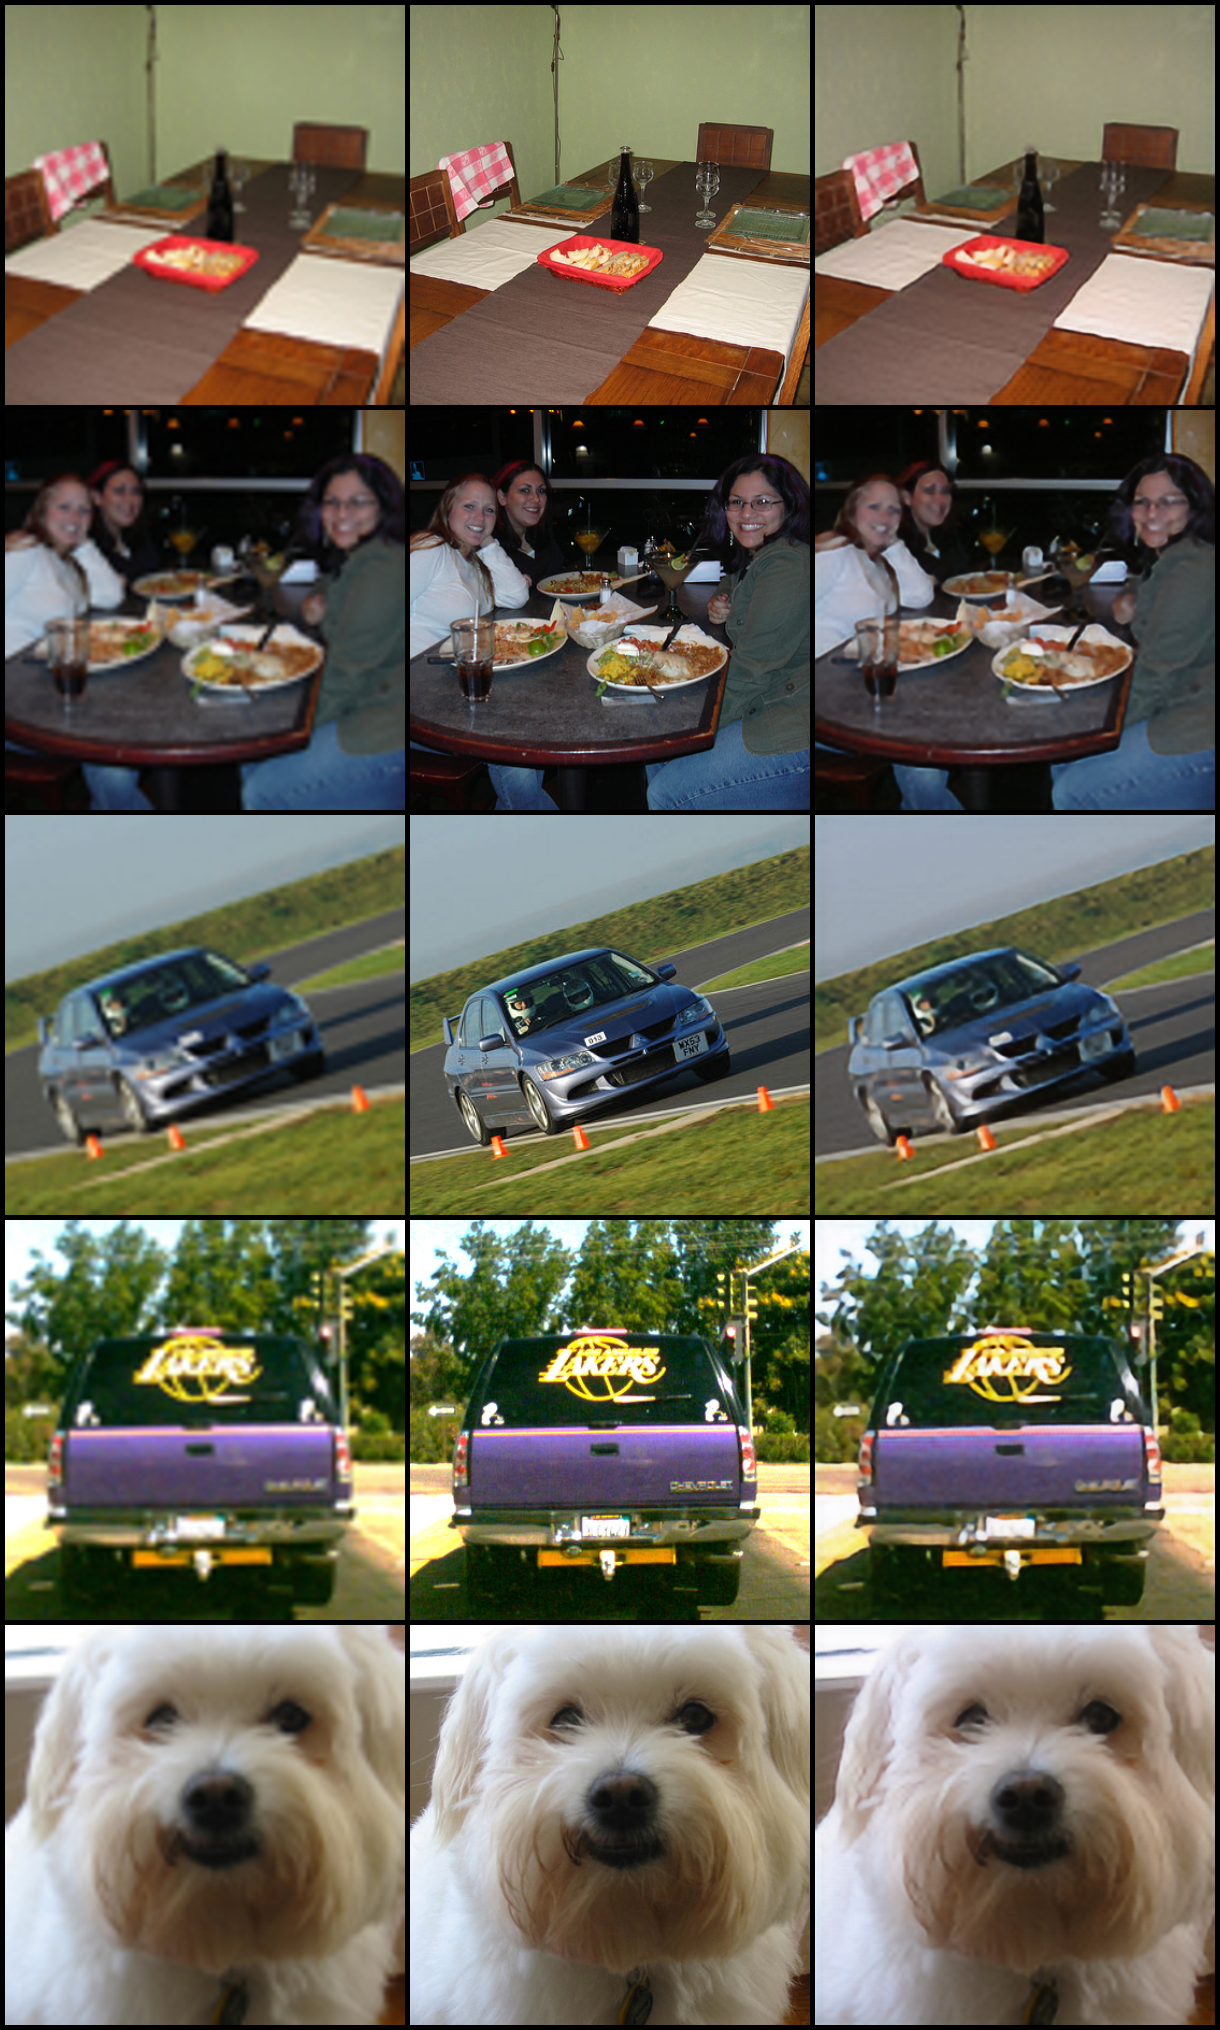
\includegraphics[width=\linewidth, height=\imageheight, clip, keepaspectratio]{epoch_11_index_10.png}%
  %     % Some sample images, low resultion, upsampled by our net(s), original high resolution.
  %   }
    
  % \end{subcolumns}
  % % now the keypoints of our project
  
  \block[]{Key Points}{%
    \begin{itemize}
    \item Networks learn even without discriminator
    \item VGG1619 performs considerably better than VGG16
    \item Training works without discriminator
    \item The discriminator is hard to train
    \item Image metrics don't change much, but the images still improve
    % \item Seemingly the training is faster with the use of a
    %   discriminator.
    % \item Metrics do not change significantly after some training but
    %   the images get better
    % \item In some settings the discriminator ``dies'' but images still
    %   improve
    % \item Discriminator loss is extreme, either very low or very
    %   large; the transition is rapid
    % \item Training the networks is tricky, discriminator ``dies''
    %   often
    % \item Visually the images change very much at beginning of
    %   training
    % \item The visual perception of the images changes for a long
    %   training time. Details added at late stages make the images seem
    %   more like actual photographs.
    % \item We could not see the large jumps for the discriminator that
    %   was shown in the paper.
    \end{itemize}
  }


  
\end{columns}


\node [text width=0.6\textwidth,above right] at (bottomleft) {% the bottomleft coordinate is defined by the class
\setcounter{footnote}{0}%
\printfootnote{\url{http://www.pascal-network.org/challenges/VOC/voc2012/workshop/index.html}} % ipsum is the text of the footnote
\printfootnote{\url{https://data.vision.ee.ethz.ch/cvl/DIV2K/}}
  };
\end{document}
